Para los test se han usado dos herramientas, el framework de testing que proporciona django rest framework sobre el framework de testing de django y POSTMAN. Todos los test que se han realizado han sido de integración.

\subsection{Django rest framework test suit}
\label{drf_test}
Para realizar test de integración automatizados se ha usado la suit que proporciona django rest framework, esta suit consta de la clase APITestCase, que permite ejecutar los test con el comando incluido en el managment.py, managment.py es una herramienta que proporciona django que permite programar tareas que se ejecutan mediante el comando ./managment.py \textit{command} en la terminal, para este caso concreto podremos ejecutar todos los test mediante el comando ./management.py test, luego podemos concretar el test que queremos ejecutar añadiendo test.\textit{nombre del test}. Los test implementados con la clase APITestCase constan de dos operaciones principales, setUp y tearDown, setUp se ejecuta antes de cada test y se puede usar para establecer el entorno con los datos deseados y tearDown se ejecuta después de cada test y podemos devolver la el entorno a su estado inicial, para no crear efectos de lateralidad entre los test (i.e. que la ejecución de un test afecte a al resultado de otro).\\
Para inicializar los test con diferentes datasets que prueben el mayor numero de pruebas posibles se ha logrado creando la clase setup\_env. En esta clase se encuentran todos los enviroments que los test puedan necesitar, esta clase se ha creado para mejorar la reusabilidad y escalabilidad de los test.\\
A continuación se adjunta el código de un test de integración como ejemplo.
\begin{lstlisting}
	class endpointsTestCase(APITestCase):

    def setUp(self):
        self.setup = setup()
        self.setup.clean_up()
        self.setup.setup()

    def tearDown(self):
        self.setup.clean_up()

    def test_get_person_serach(self):
        '''
        search person
        '''
        url = reverse(
            'person-detail',
            kwargs={'id': self.setup.person1.id}
        )
        url += 'search/'
        response = self.client.get(
            url,
            format='json',
            HTTP_AUTHORIZATION=self.setup.token_bearer
        )
        print response
        self.assertTrue(status.is_success(response.status_code))
\end{lstlisting}

Este caso es un test muy simple, comprueba que realmente el endpoint retorna el status\_code esperado, en este caso un 201.

Estos tipos de test de tan alto nivel y tan poco pormenorizados en lenguajes no compilados como python son de gran importancia ya que la mayoría de fallos surgen en tiempo de ejecución. Lógicamente igual que se testan los endpoints también se testan las funciones importantes y se comprueba que retornen el resultado esperado según un setup determinado.\\
Una vez pasados los test vemos el mensaje de la figura \ref{fig:test}
\begin{figure}[ht!]
\center
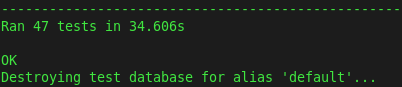
\includegraphics[scale=1.3]{screenshots/test.PNG}
\caption{Test realizados con la django}
\label{fig:test}
\end{figure}
\newpage
\subsection{POSTMAN}
Por otro lado se han realizado test a más alto nivel con la herramienta POSTMAN, con esta herramienta podemos hacer llamadas a nuestra API simulando que somos un tercero que la esta usando. POSTMAN también proporciona herramientas de automatización de los test mediante las colecciones de llamadas.\\
Primero nos fijaremos en las colecciones, nos aparecen en el panel lateral y es donde se almacenaran nuestros test (Figura \ref{fig:postman_coll}). 
\begin{figure}[ht!]
\center
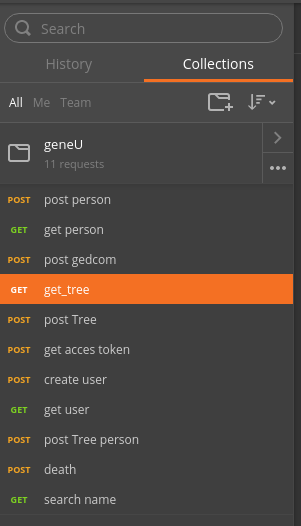
\includegraphics[scale=0.7]{screenshots/postman_collections.PNG}
\caption{Vista de las colecciones en la interfaz de POSTMAN}
\label{fig:postman_coll}
\end{figure}
\newpage
En la figura \ref{fig:postman_test} podemos ver como se ven los test, estos son ejecutados con la \textit{Send} o cuando ejecutamos todos de manera automática.
\begin{figure}[ht!]
\center
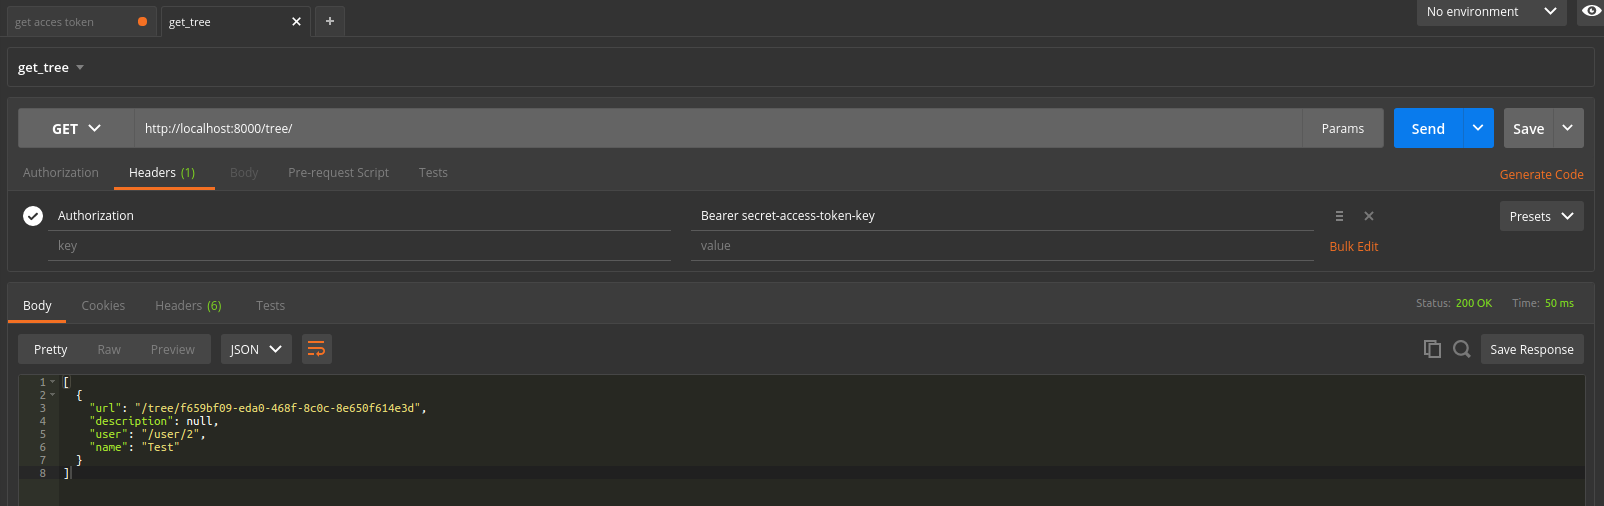
\includegraphics[scale=0.5]{screenshots/postman_test.PNG}
\caption{Vista de un test en la interfaz de POSTMAN}
\label{fig:postman_test}
\end{figure}

Para facilitar la ejecución de los test con POSTMAN se ha creado un nuevo comando en el managment.py, herramienta que hemos visto en el apartado anterior \ref{drf_test}, con el fin de primero limpiar todo el envirmoent y luego inicilizarlo con un dataset.
Este es el codigo:
\begin{lstlisting}
class Command(BaseCommand):
    help = "clean all nodes and relations of the db"

    def add_arguments(self, parser):
        parser.add_argument('-s', '--set', nargs='?', help='...')

    def handle(self, *args, **options):

        subprocess.call(["python", "manage.py", "clean_neo_db"])
        subprocess.call(["python", "manage.py", "setup_loc_environ"])
        subprocess.call(["python", "manage.py", "setup_date_environ"])

        subprocess.call(["python", "manage.py", "reset_db"])
        subprocess.call(["python", "manage.py", "migrate"])
        subprocess.call([
                            "python", "manage.py", "createsuperuser",
                            "--username=admin", "--email=admin@geneu.com"
                        ])
        set_nj4 = ["python", "manage.py", "set_neo4j"]
        if options['set']:
            set_nj4 += ["-s", options['set']]
        subprocess.call(set_nj4)
\end{lstlisting}

\begin{description}
\item[clean\_neo\_db]: Wipea la base de datos de neo4j
\item[setup\_loc\_environ]: Efectúa las inicializaciones pertinentes para poder trabajar con el modulo.
\item[setup\_date\_environ]: Efectúa las inicializaciones pertinentes para poder trabajar con el modulo.
\item[reset\_db]: Wipea la base de datos sql.
\item[migrate]: Inicializa la base de datos sql para poder trabajar con ciertos módulos que lo requieran.
\item[createsuperuser]: Crea un superusuario.
\item[set\_neo4j]: Inicializa la base de datos neo4j con un juego de pruebas.
\end{description}
*Los comandos clean\_neo\_db, setup\_loc\_environ, setup\_date\_environ, set\_neo4j también se han tenido que crear para poder llevar a acabo todo el proceso. Los demás vienen incluidos en Django.